
\documentclass[11pt, aspectratio=169]{beamer}
\usepackage{templates/beamerthemeICubebase}

% Remove navigation bar
\setbeamertemplate{navigation symbols}{}
% Tikz package
\usepackage{tikz}
\usetikzlibrary{positioning}
\usetikzlibrary{matrix}

\usepackage[export]{adjustbox}
\usepackage{booktabs}
\usepackage{siunitx}
\usepackage{amssymb}
\usepackage{xmpmulti}
\usepackage{caption}
\usepackage[absolute,overlay]{textpos}
\setbeamertemplate{footline}[frame number]
\usepackage{graphicx}
\graphicspath{{figures/},{logos/}}

% Make links show up as coloured
\hypersetup{
  colorlinks = true,
  allcolors = black,
  urlcolor = blue,
}
%\definecolor{lucid-blue}{RGB}{41, 170, 225}
%\setbeamercolor{frametitle-left}{fg=unistra}
%\setbeamercolor{frametitle}{fg=white}
\setbeamerfont{frametitle}{size=\Large}
\setbeamerfont{framesubtitle}{size=\small}
\newcommand{\fullframeimage}[1]{
	\begin{center}%
		\includegraphics[max width = \textwidth, max height=0.8\textheight]{#1}%
	\end{center}
}

\setbeamercolor{frametitle}{fg=white,bg=unistra}

%\let\emph\relax % there's no \RedeclareTextFontCommand
\DeclareTextFontCommand{\emph}{\color{slide-color}}
\setbeamercolor{background canvas}{bg=white!20}
%\colorlet{slide-color}{unistra}


\title{Laboratoire des sciences de l'ingénieur, de l'informatique et de l'imagerie}
\subtitle{ICube, UMR 7357}
\author{L. Barbé}
\institute{Plateforme Imagerie, Robotique et Innovation en Santé}
\date{\today}


% Bibliography
% Uncomment and upload your own references if you so please.
% \usepackage[citestyle=authoryear,bibstyle=numeric,hyperref,backend=biber]{biblatex}
% \addbibresource{references.bib}
% \bibhang1em
%\titlegraphic{\includegraphics[height=1cm]{logos/icube/icube-png.png}}


\begin{document}

\selectlanguage{french}

%\frame{\titlepage}
\begin{frame}[plain]
    \begin{tikzpicture}[remember picture,overlay]
    % Background image
    \node[above right, align=center,inner sep=0pt] at (current page.south west)
    {
        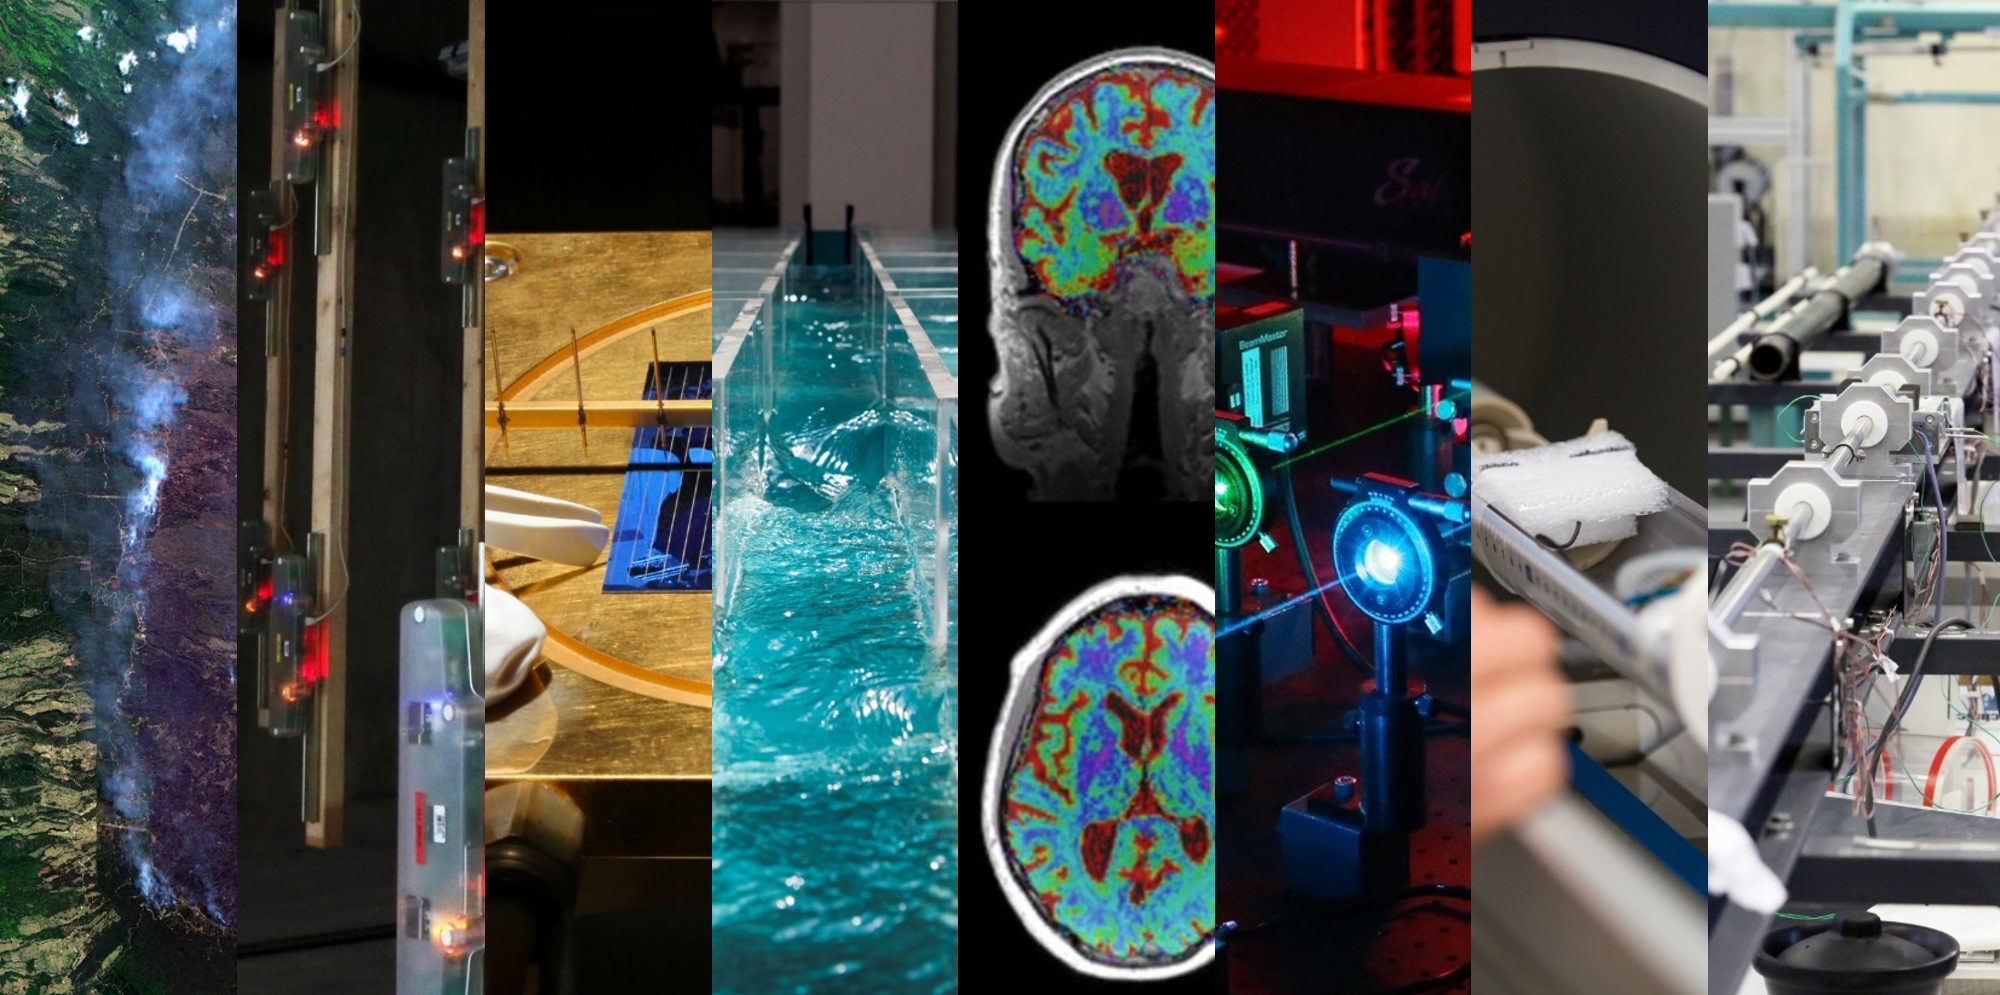
\includegraphics[width=0.95\paperwidth]{image_fond.png}
    };
        
    % Title & Subtitle
    \node
    [
        above=0.5cm,
        align=left,
        fill=unistra,
        rounded corners,
        inner xsep=15pt,
        inner ysep=10pt,
        minimum width=0.85\textwidth,
        text width=0.8\textwidth,
        fill opacity=0.7,
        text opacity=1,
        text=white
    ] (title) at (current page.center)
    {
        \Large \textbf{\inserttitle }  \\[5pt]
        \small \insertsubtitle
    };
    \node
    [
        below=0.5cm,
        align=left,
        fill=unistra,
        rounded corners,
        inner xsep=15pt,
        inner ysep=10pt,
        minimum width=0.7\textwidth,
        text width=0.6\textwidth,
        fill opacity=0.7,
        text opacity=1,
        text=white
    ] (subtitle) at (title.south)
    {
        \large \insertinstitute  \\[5pt]
    };
    % Author 
    \node[  below=0.5cm,        
            align=left,
            fill=unistra,
            rounded corners,
            inner xsep=15pt,
            inner ysep=10pt,
            minimum width=0.7\textwidth,
            text width=0.6\textwidth,
            fill opacity=0.7,
            text opacity=1,
            text=white
    ] (author) at (subtitle.south){\insertauthor};
    % Date
    \node[below=0.5cm,             
    align=left,
    fill=unistra,
    rounded corners,
    inner xsep=15pt,
    inner ysep=10pt,
    minimum width=0.7\textwidth,
    text width=0.6\textwidth,
    fill opacity=0.7,
    text opacity=1,
    text=white] (date) at (author.south){\large \today};
    % Logo

     \node
    [
        below right =0.25cm and 0.5cm
    ] at (current page.north west)
    {
         \includegraphics[height=1.5cm]{icube/icube-png.png}
    };
    \node
    [
        below left =0.25cm and 0.25cm
    ] at (current page.north east)
    {
        \includegraphics[height=0.6cm]{inria/inr_logo_rouge.png}
    };
    \node
    [
        below left =0.25cm and 2.2cm
    ] at (current page.north east)
    {
        \includegraphics[height=0.6cm]{engees/ENGEES_CMJN_png.png}
    };
    \node
    [
        below left =0.25cm and 3.5cm
    ] at (current page.north east)
    {
        \includegraphics[height=0.6cm]{insa_strasbourg/Logo_INSAvilleStrasbourgCourt-pantone_marge.jpg}
    };
    \node
    [
        below left =0.25cm and 5.0cm
    ] at (current page.north east)
    {
        \includegraphics[height=0.6cm]{cnrs/LOGO_CNRS_BLEU.png}
    };
    \node
    [
        below left =0.25cm and 6cm
    ] at (current page.north east)
     {
         \includegraphics[height=0.6cm]{unistra/signature-universite-minimale-couleur_03.png}
    };
    \end{tikzpicture}
    %\titlelogoe{}
\end{frame}

\begin{frame}
    \frametitle{ICube, un laboratoire pluridisciplinaire}
    \framesubtitle{Une force de recherche majeure à Strasbourg (760 personnes)}

    \begin{block}
        ICube existe depuis le 1$^{er}$ Janvier 2013 :
        \begin{itemize}
            \item un laboratoire de recherche en \textbf{ingénierie}, en \textbf{informatique} et en \textbf{imagerie} avec comme secteurs d'activités privilégiés la \textbf{santé}, l'\textbf{environnement} et le \textbf{développement durable}.
            \item une unité mixte de recherche (UMR7357) sous la cotutelle de l’\textbf{université de Strasbourg}, du \textbf{CNRS}, de l’\textbf{INSA Strasbourg}, de l’\textbf{ENGEES} et de l’\textbf{INRIA Grand Est}.
        \end{itemize}
    \end{block}
 

    % \vfill
    % \begin{figure}
    %     \centering
    %     {\def\svgwidth{0.7\textwidth}\footnotesize\input{figures/standard_BelleII_decay.pdf_tex}}
    %     \caption{Hehe particles go BRRRR}
    %     \label{fig:my_label}
    % \end{figure}
\end{frame}
\begin{frame}
    \frametitle{La plateforme IRIS}
    \framesubtitle{Imagerie, Robotique et Innovation en Santé}
    \begin{block}{Le rôle}
    La plateforme IRIS  offre les moyens et un support à la recherche en Imagerie, en Robotique et l'Innovation pour la Santé
    \end{block}
    \begin{block}{Nos missions}
        Fournir une expertise et un environnement à la fois matériel et logiciel permettant :
        \begin{itemize}
            \item le développement et l'optimisation de protocole d'imagerie biomédicale (IRM, Ultrason, imagerie optique, etc.) ;
            \item l'élaboration et l'évaluation de dispositifs pour l'imagerie médicale et biomédicale multimodale ;
            \item le développement d'assistant robotique pour le GMCAO (hardware et software) ; 
            \item l'analyse et le traitement des données ;
            \item la réalisation d'études cliniques et pré-cliniques ;
            \item essais biomécaniques; 
        \end{itemize}
    \end{block}
\end{frame}
%=====================================================================================================================================
\begin{frame}
    \frametitle{La plateforme IRIS}
    \framesubtitle{Un emplacement unique}
    Située dans l'enceinte de l'hôpital Civil de Strasbourg, répartie sur 3 sites avec près de 1500 m$^2$ de surface :
    \begin{itemize}
        \item Nouvel Hôpital Civil (NHC), IRM Interventionnelle dans le service d'imagerie interventionnelle du Pr. Gangi ;
        \item Institut Hospitalo-Universitaire (IHU), plateau technique robotique et mécatronique ;
        \item Institut de Physique Biologique (IPB), imagerie homme et pré-clinique, biomécanique et informatique.
    \end{itemize}
    \begin{figure}[!h]
        \centering
            \includegraphics[height=4cm]{img/plan-acces.png.png}
    \end{figure}
\end{frame}
%=====================================================================================================================================
\begin{frame}
    \frametitle{La plateforme IRIS}
    \framesubtitle{Réseaux et labelisation}
    \begin{itemize}
        \item IRIS est impliquée dans plusieurs réseaux régionaux et nationaux
    \end{itemize}
    \begin{columns}
        \column{0.3\textwidth}    
        \begin{figure}[!h]
            \centering
                \includegraphics[height=0.7cm]{logos/reseaux_labelisation/nyg_nouleur-2.png}
                \caption*{FHU Neurogeneti$\Phi$cs, Strasbourg}
        \end{figure}  
        \column{0.3\textwidth}    
        \begin{figure}[!h]
            \centering
                \includegraphics[height=0.7cm]{logos/reseaux_labelisation/logo_FMTS.jpg}
                \caption*{Fédération de Médecine Translationnelle de Strasbourg}
        \end{figure}  
        \column{0.3\textwidth}    
        \begin{figure}[!h]
            \centering
                \includegraphics[height=0.7cm]{logos/reseaux_labelisation/neuropole_photo_large.jpg}
                \caption*{Neuropole - Pôle des Neurosciences de Strasbourg}
        \end{figure}              
    \end{columns}
    % ROBOTEX 2.0
    \begin{columns}
        \column{0.3\textwidth}
            \begin{figure}[!h]
                \centering
                    \includegraphics[height=0.7cm]{logos/reseaux_labelisation/ROBOTEX2.0-V1.png}
            \end{figure} 
        \column{0.7\textwidth}
            ROBOTEX2.0 réseau des plateformes nationales  de robotique.
    \end{columns}
    % FLI
    \begin{columns}
        \column{0.3\textwidth}
            \begin{figure}[!h]
                \centering
                \includegraphics[height=0.7cm]{logos/reseaux_labelisation/FLI_Logotype_Coul-5cm.jpg}
            \end{figure} 
        \column{0.7\textwidth}
            FLI, France Life Imaging.
    \end{columns}
    % IBISA
    \begin{columns}
        \column{0.3\textwidth}
            \begin{figure}[!h]
                \centering
                \includegraphics[height=0.7cm]{logos/reseaux_labelisation/IBISA.png}
            \end{figure} 
        \column{0.7\textwidth}
            IBISA, Infrastructure en Biologie, Santé et Agronomie
    \end{columns}
    % CARNOT TSN
    \begin{columns}
        \column{0.3\textwidth}
            \begin{figure}[!h]
                \centering
                \includegraphics[height=0.7cm]{logos/reseaux_labelisation/logo Carnot TSN.jpg}
            \end{figure} 
        \column{0.7\textwidth}
            CARNOT, Télécom \& Société Numérique
    \end{columns}
\end{frame}

%=====================================================================================================================================
\begin{frame}
    \frametitle{La plateforme IRIS}
    \framesubtitle{6 pôles d'expertises}
    \begin{itemize}
        \item Neuro-Imagerie Homme :
        \item Imagerie Pré-Clinique :
        \item Imagerie Interventionnelle :
        \item Biomécanique :
        \item Robotique :
        \item Informatique et Traitement d'Images :
    \end{itemize}
\end{frame}
\begin{frame}{Le pôle Robotique}
    
\end{frame}
% One way to make a slide


\end{document}
